\chapter{Implementation}

In the previous chapter we explored a methodology that proposes how to leverage common points between \acf{PLE} and \acf{MDE} for domain analysis, requirement engineering, and feature modelling. We have also introduced a language, \tool, to demonstrate how requirement modelling can be combined with feature modelling to improve traceability via a defined hierarchy between features and requirements.

In this chapter we explore an implementation of \tool\ that shows the capability of tool support for the language. Through this implementation, we attempt to show capability of automatic traceability generation and maintenance from good modelling practice and feasibility of iterative and incremental development using the proposed methodology with tool support.

As a proof of concept, we have implemented a \ac{DSL} using Sirius~\cite{viyovic2014sirius} and Xtext~\cite{eysholdt2010xtext} to show the feasibility of automated traceability between features and requirements. This is a core component of the methodology as we require the means to specify feature models and requirements to capture their interrelationships to enable automated traceability. By implementing a \ac{DSL}, we can enforce syntactic and semantic rules defined from the metamodel to create verifiable models to support incremental and iterative development.

The tool for \tool\ also provides us an environment where we have been exploring potential composition strategies. We anticipate that as a result of designing the language of \tool\ to be focused on feature-requirement traceability there may be some side effects. By implementing the language in a tool, we can explore some of these side effects such as the impact it may have on composition techniques from \ac{PLE}. Some modifications may be required as a result of the relationship we have introduced between features and requirements. 

%Though not automated at this time, the facilities in \tool\ were sufficient as a proof of concept to allow further development for composition in the future.

\section{Implementation Objectives}

\subsection{Goals and Limitations}

In figure~\ref{fig:CyclicL_goals} we capture some anticipated goals for our end-users. In conjunction with our own objectives, we use these to support our high-level requirements for \tool. At the time of writing the scope of \tool\ is currently only focused on the traceability portion of the methodology we have scoped user goals to be after they have completed an independent domain analysis. We assume that users will complete the other steps of this methodology (goal diagrams, \ac{UCD}) using other means prior to or as part of an iterative process when using \tool. This is a limitation of \tool\ for now as we do not currently support modelling or traceability from the domain analysis to the identified features and requirements. We strongly encourage that users complete the prior steps of domain analysis before modelling the features and requirements as it helps the development process to build a better conceptual model and understanding of the intended product~\cite{kang1990feature}.

\begin{figure}
	\centering
	\includesvg[width=\textwidth]{CyclicL_goals}
	\caption{Anticipated goals of users for \tool.}
	\label{fig:CyclicL_goals}
\end{figure}

We have a couple of key goals we are aiming to satisfy by implementing a tool for \tool. 

\begin{itemize}
	\item Enforce syntax and semantic rules of \tool\ when creating models.
	\item Explore impacts of traceability generation and maintenance when creating and changing models within the tool.
	\item Enforce automated traceability as a side effect of model creation.
	\item Explore the impact of feature-requirement traceability on both feature modelling and requirement modelling.
	\item Reuse as many specifications and definitions from previous work as possible.
\end{itemize}

We expect the main users of the tool to be engineers, primarily but not limited to software engineers. To be successful, the tool needs to allow users to create feature models so they can define their product families. It also needs to have a way to define requirements. Since \tool\ is also an implementation of the methodology the tool also needs to implement the relationship we have defined between features and requirements. Finally, since we want to support iterative and incremental development, the tool for \tool\ also needs to have some way to enhance the process of generating and maintaining traceability matrices for requirements and features. Finally, the implementation needs to be robust with respect to change to support future changes such as traceability to uses cases and goals or other automated processes such as change impact analysis and product composition.

Based on our objectives, the tool for \tool\ has two main modelling environments that are distinct and connected as demonstrated in the abstract syntax in figures~\ref{fig:feature_mm}, \ref{fig:req_canvas_mm1}, and~\ref{fig:req_canvas_mm2}. The first is the feature modelling half of the tool. The purpose of this modelling environment is to allow the user to build their product family; what are the features and how are they related. The second modelling environment is the requirement canvas. This portion of the tool enables users to specify their requirements, associate requirements to design elements, and assign reviewers and test cases to requirements. This is where the traceability is captured between the feature and various aspects of the requirements. 

Another objective we had during development was reuse. As we were exploring and implementing traceability, and in the spirit of \ac{PLE}, we were trying to identify as many reusable aspects as possible from previous specifications and implementations of tools as we could. Thus, \tool\ is also inspired by FeatureIDE~\cite{kastner2009featureide, thum2014featureide} and GEARS~\cite{GEARS} for their abstract and concrete syntaxes. This prevented us from having to reinvent how to build a feature modelling tool so we could focus more efforts on the requirement canvas and the traceability matrices.

\subsection{Requirements}
We extracted high-level requirements from previous work in building a product line and requirements for a coffee cup to guide initial development plans for \tool~\cite{chiang2024mapping}. We also have the goal of supporting iterative and incremental development life-cycles. We generally define an iterative change as a change based on feedback from later stages of development or stakeholders. These are usually larger changes that may arise cycling between phases of development. In the context of \tool, we want to generate and maintain traceability between features and requirements as users iterate between feature modelling and requirement modelling. Examples of an iterative change can include a new version of a development artifact or a redesign of a development artifact. Incremental changes are changes that are usually smaller in scope, and bound within a single development phase, such as feature modelling \textit{or} requirement modelling. Examples of an incremental change can be a refactoring change, updating a definition, or changing a connection between components. While we have been using these definitions to guide our development philosophy, this may not be a shared definition by others. This may present a challenge to the adoption or usage of \tool. Therefore, we included ease of use and adoption as another goal. Our initial list of requirements was as follows:

%relative to an incremental change. 

\begin{itemize}
	\item Tool shall provide the user with an environment for defining requirements.
	\item Tool shall provide the user with an environment for defining features.
	\item Tool shall allow the user to specify design elements.
	\item Tool shall allow the user to relate one or more requirements to one or more design elements.
	\item Tool shall allow the user to use features to capture and own requirements.
	\item Tool shall automatically create and maintain a traceability matrix.
	\item Tool shall facilitate iterative development of the requirements canvases (\textit{note:} this remains as ongoing work).
	\item Tool shall facilitate incremental development of the requirements canvases.
	\item Tool shall aim to promote familiarity and ease of use to increase rate of adoption.
\end{itemize}

Along with these requirements, we also use the prior specifications for feature-requirement encapsulation. We treat the requirements encapsulated by a feature as attributes and are considered feature requirements, thus scoped by the feature. As the exploration of requirement modelling started with the requirement diagrams from SysML, we reused as much as possible from the original specification. We then focused more on traceability aspects and integration with feature modelling, diverging from the original specification until we ended up with what we now refer to as our requirement canvas. For a rough idea of what we wanted the requirement canvases to look like we sketched requirements for a disposable coffee cup with a handle, shown in Figure \ref{fig:CoffeCup_ReqModel}.

\begin{figure}[hbt!]
	\centering
	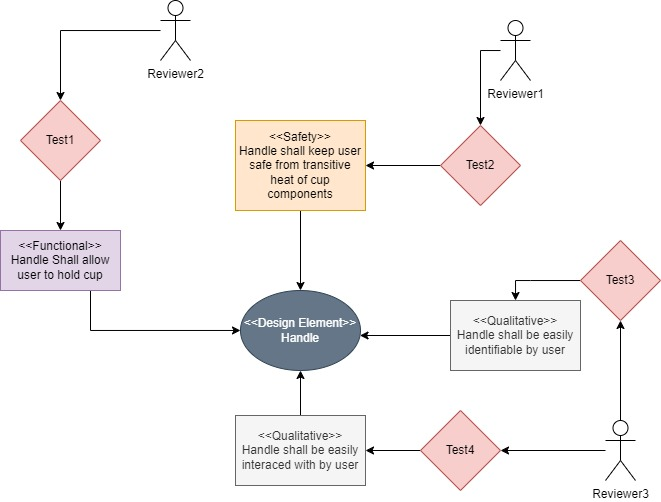
\includegraphics[width=\columnwidth]{Figures/CoffeCup_ReqModel.jpg}
	\caption{Example of a requirement canvas concrete syntax. The example uses a disposable coffee cup with a handle as the focus of the diagram.}
	\label{fig:CoffeCup_ReqModel}
\end{figure}

\section{Abstract Syntax}
\label{sec:Abstract_Syntax}

The metamodel shown in figure~\ref{fig:metamodel} is what we used as a specification for building the tool for \tool. The abstract syntax can be roughly divided into two main portions; the feature model shown in figure~\ref{fig:feature_mm} and the requirement canvas shown in figure~\ref{fig:req_canvas_mm1} and~\ref{fig:req_canvas_mm2}. This is inline with our requirement decisions for \tool. The requirement canvas portion of the metamodel is not a complete implementation of the SysML specification for requirement diagrams. We decided to implement enough to allow us to model requirements sufficiently to get traceability. 

\subsection{Feature-Requirement Encapsulation}
To enable features to encapsulate requirements, the \texttt{FeatureEntity} class inherits from the \texttt{Requirement\_Canvas} class. This implementation is what allows the features to encapsulate the requirements. We chose the inheritance relationship as it makes the features share the semantically equivalent to a requirement canvas while also allowing us to define a feature independent of a requirement canvas syntactically. Using another relationship for the implementation, such as a composition relationship, would have added a strict ownership semantic that we did not find added any value and instead added an extra layer of abstraction between features and requirements that ended up cluttering the traceability with useless information. Through this inheritance relationship the features own the requirement directly without any abstraction. Further, the inheritance specification forces a 1-1 relationship between the requirements and the feature meaning every new set of requirements will require a new feature to be encapsulated, reinforcing the convention of a unique feature per unique set of requirements. This relationship is highlighted in figure~\ref{fig:requirement_feature_inheritance}.

\begin{figure}
	\centering
	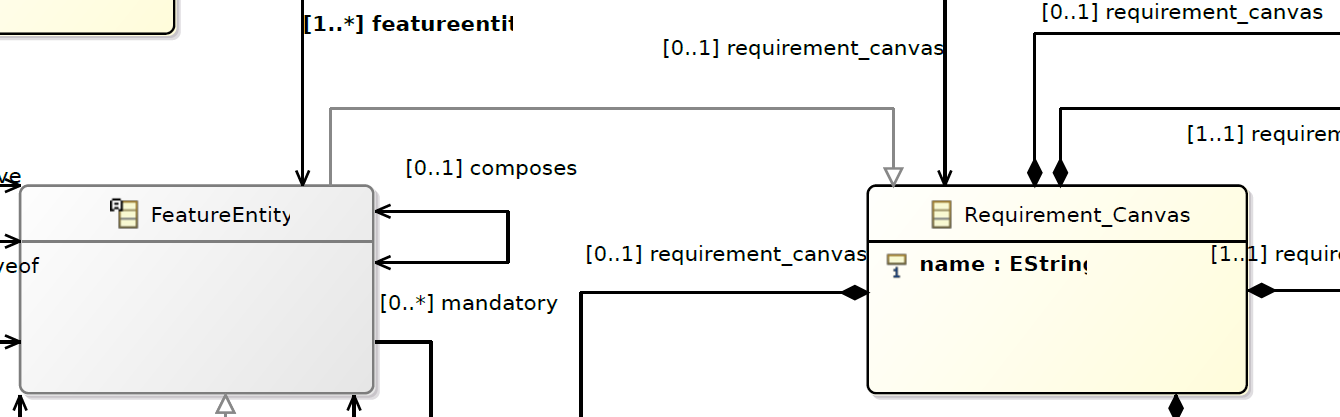
\includegraphics[width=\textwidth]{requirement_feature_inheritance.png}
	\caption{Specification of the inheritance relationship between the requirement canvas and the feature entities in \tool.}
	\label{fig:requirement_feature_inheritance}
\end{figure}

\subsection{Feature Model Specification}

The feature modelling specification of the tool is loosely inspired by the formal approach from Peter H\"{o}fner \textit{et al}~\cite{hofner2006feature,hofner2011algebra}, with a small extension to account for requirement encapsulation. We use this specification instead of making a new one to leverage previous proofs and work done on formal specifications for feature modelling. It saved us time and let us begin development much sooner. We consider the relationship between features and requirements within a product family as shown in figure~\ref{fig:spec}. By using this definition, we treat each feature as a set of requirements such that every requirement within the feature is unique. As stated in the definition however, it does not account for duplicate requirements in separate feature elements. This is something that will be addressed in future iterations. 

Specifying the hierarchy between features are requirements both in a metamodel and using a set theory approach gives us a better understanding for the mechanisms involved between the two entities. The idea is that this will help with specifying and implementing mechanical processes, for example change impact analysis, in the future using a formalized language like the Object Constraint Language (OCL)~\cite{richters2002ocl, cabot2012object}, or another formal approach. This should help with validation of the mechanism and streamline development as we can use one of it's derivatives baked into Eclipse like \ac{EVL} or \ac{AQL}.

\begin{figure}
	\begin{align}
		\text{Let } \mathbb{F} \text{ be a set of arbitrary elements that we call features.}\\
		\text{We can call a collection (set) of features a product.}\\
		\text{The set of all possible products is } \mathbb{P} \overset{\mathrm{def}}{=} \mathcal{P}(\mathbb{F})\\
		\text{A collection of products (an element of } \mathcal{P}(\mathbb{P})\text{)}\\
		\text{is called a product line (or product family)}\\
		\text{This model does not capture feature duplication}\\
		\text{Let } \mathbb{R} \text{ be a set of arbitrary elements that we call requirements.}\\
		\text{We can call a collection (set) of requirements a feature.}\\
		\text{The set of all possible features is: } \mathbb{F} \overset{\mathrm{def}}{=} \mathcal{P}(\mathbb{R})\\
		\text{This model does not capture requirement duplication.}
	\end{align}
	\caption{Definition of the relationship between features and requirements.}
	\label{fig:spec}
\end{figure}

There are three defined relationships for features; mandatory, alternative, and optional. These are specified with bidirectional references to allow visibility in either direction from any feature. This decision was made to enhance the traceability available in the modelling environment and simplify development for the traceability matrices. The multiplicities are also defined with 0..1 at the top end to limit how the feature composition will work. This limits how many nodes a leaf element can be connected to, constraining what models can be built and simplifying the feature composition. We also highlight the requirement set owned by the null feature based on the composition relationship from \texttt{RMDL\_Project} to \texttt{Requirement\_Canvas}. The justification for this structure is to provide an extra space for requirement specification that can later be refined by cutting and pasting the  requirements into a canvas encapsulated by a proper feature. To prevent cluttering instantiated projects with too many disconnected drawing spaces we limit the multiplicity to [0..1].

%Further, our specification allows for another interesting scope. We can have the 'null feature' scope. This is the requirement canvas that isn't owned by any feature model. This is enabled via the composition relationship from the project root class down to the requirement canvas class, shown in figure~\ref{fig:null_req_canvas.png}. Due to cardinality of 0..1, CyclicL affords the end user the option to create a requirement canvas belonging to no feature.
%
%\begin{figure}
%	\centering
%	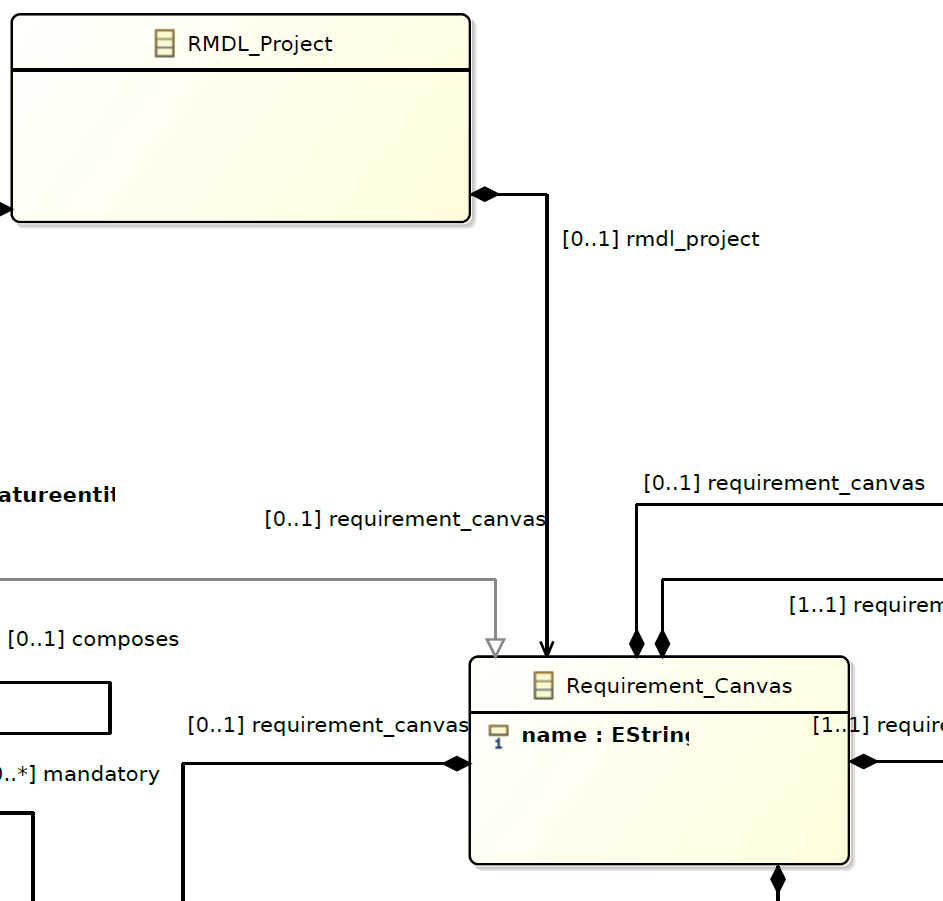
\includegraphics[width=\textwidth]{null_req_cavnas.png}
%	\caption{Specification for the requirement canvas owned by null. This provides a sort of drawing space or backlog for requirements that users have not yet sorted into a feature.}
%	\label{fig:null_req_canvas}
%\end{figure}

%The requirement canvas also has a containment relationship with the model root, \texttt{RMDL\_Project}. This is carried over from earlier development and was left in the tool, for now, to allow users to define a requirement canvas for the entire system they are specifying without being tied to specific features. 

%. Thus, every feature in the feature model can become a requirement canvas, allowing us to capture the requirements for each feature as attributes of said feature. 

\subsection{Requirement Canvas Specification}

The requirement canvas portion of \tool\ that was inspired by requirement diagrams from SysML~\cite{sysml2019omg}, however we did not end up implementing it according to its original specification. The main reason for the divergence was due to our focus on implementing the feature-requirement hierarchy and developing for feature-requirement traceability specifically. As a result, we decided to iterate on requirement diagrams as a means of exploration for traceability and requirement specification leading to the inception of the requirement canvas. In the process of exploring we made several decisions both at the requirements and design level for \tool\ that led to its state at the time of writing. This includes the classifications for functional and non-functional requirements, the graphical syntax implemented, and the specification language embedded in the model. We explain these differences in the following passages.

Next, for the requirements in the requirement canvas, we identified four requirement categories; \texttt{Functional}, \texttt{Qualitative}, \texttt{Constraint}, and \texttt{Safety}. These are shown in figure~\ref{fig:req_type}.

\begin{figure}[hbt!]
	\centering
	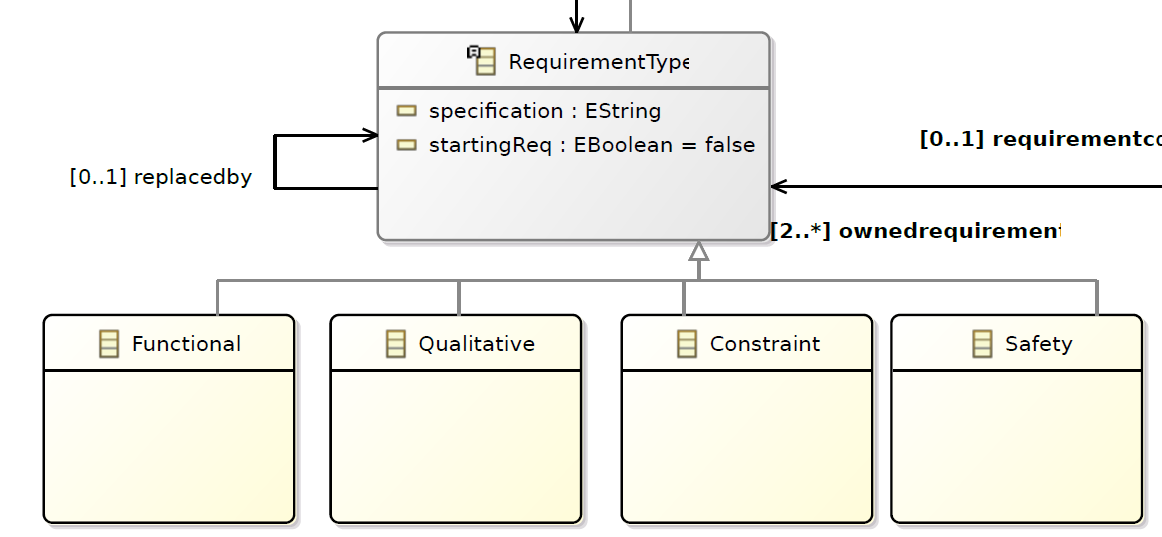
\includegraphics[width=\textwidth]{req_type.png}
	\caption{Specification for the 4 requirement types in \tool.}
	\label{fig:req_type}
\end{figure}

Functional requirements follow their traditional definition; things that a product or system must do. Qualitative requirements are identified as requirements that affect the way a product or system accomplishes its function. These include the look, feel, usability, humanity, and some performance requirements that are not categorized as functional. Constraint requirements are identified as requirements that add limitations of some type to a product or system. These include operational, environmental, maintainability, support, security, cultural, political, and legal requirements. These requirement definitions can be found in James and Suzanne Robertson Volere requirements~\cite{robertson2000volere}. We found a benefit for more specific categories beyond just non-functional requirement as it lets the user be more intentional with their specification. We find this especially beneficial for identifying safety requirement separate from the other traditional non-functional requirements. The safety requirement category is critical for our purposes as they identify all requirements that have to do with the safety of users or stakeholders involved in the function of a product or system. We highlight safety requirements as a separate requirement category as we want to target \tool\ towards safety-critical development. It is important to note that requirement categorization relies heavily upon system, or in \tool, feature scoping. For example, we hypothesize that in a safety feature, a safety requirement may be considered a functional requirement due to the feature scope. A functional feature, however, may contain safety requirements that are distinctly different from the functional requirements. This distinction relies heavily upon the judgement of the engineer creating the model and the model context.

We also added three more classes besides the requirements; \texttt{DesignElement}, \texttt{Review}, and \texttt{TestCase} shown in figure~\ref{fig:design_test_review}. 

\begin{figure}[hbt!]
	\centering
	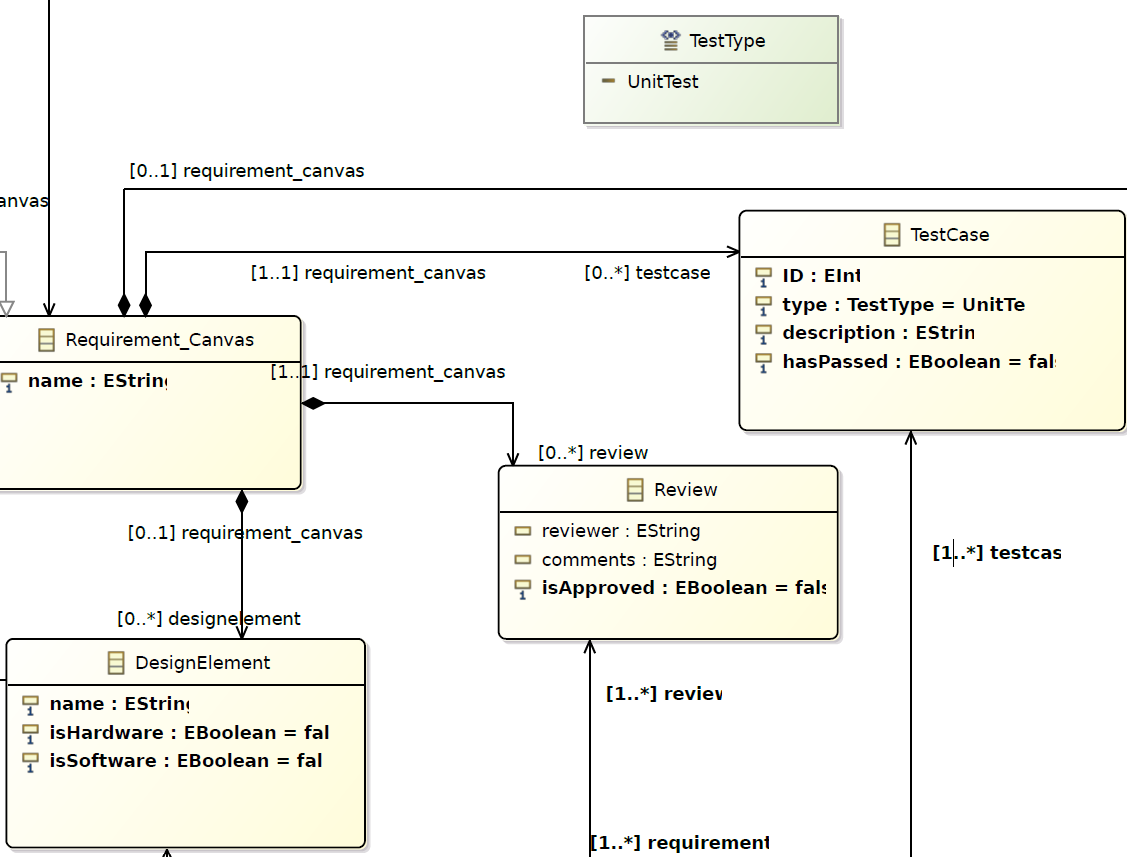
\includegraphics[width=\textwidth]{design_test_review.png}
	\caption{Specification for design, test, and review in \tool.}
	\label{fig:design_test_review}
\end{figure}

The test case and review classes are for verification and validation book-keeping respectively. We also have an enum \texttt{TestType}. This enum allows users to categorize the test users may want to apply to their requirements. At this time in development, only \texttt{UnitTest} is implemented as a type, but more can be added in future revisions. This is also one of the reasons why we include design elements within the requirement canvas. The test cases are meant to determine if a requirement has been verified against its traced design elements while the review represents if the requirement has been validated. Currently, the verification and validation are expected to happen outside of \tool\ as it was out of scope for initial development. Design elements are also meant to be black boxes as we do not want to pollute our requirement environment with design aspects. We have limited it to determining if a design element is hardware, software, or neither (undetermined when building the requirements or an integrated system). Another reason for having design elements within the requirement canvas is to allow an opportunity for future development for design generation based on the requirements specified in \tool.



%As discussed in section~\ref{sec:feat-req_traceability}, the features encapsulate the requirements via the inheritance relationship from the requirements canvas class to the feature model class. 

%This is our implementation of the hierarchy between features and requirements. Connecting these two modelling environments affords us a variety of traceability options. Scoping the traceability matrix to a single feature we can get a simple requirement traceability matrix. Scope the traceability to the product family and we can get a tabular representation of the feature model. Or, from the same scope, we can get complete traceability of all the requirements present in the product family. This includes their owning features so we can have a full list of complete traceability for all the features and requirements. We anticipate that this same mechanism can be used to generate traceability based on product instances as well.

Further, our specification allows for another interesting scope. We can have the 'null feature' scope. This is the requirement canvas that isn't owned by any feature model. This is enabled via the composition relationship from the project root class down to the requirement canvas class, shown in figure~\ref{fig:null_req_canvas.png}. Due to cardinality of 0..1, CyclicL affords the end user the option to create a requirement canvas belonging to no feature.

\begin{figure}[hbt!]
	\centering
	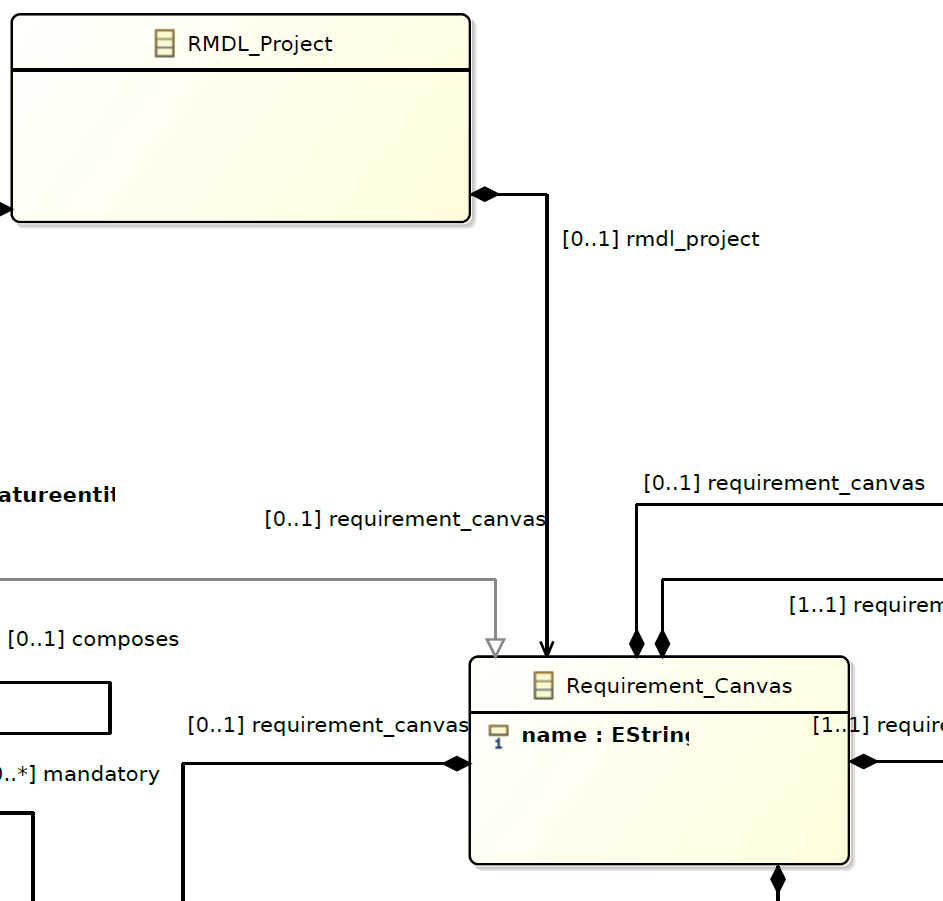
\includegraphics[width=\textwidth]{null_req_cavnas.png}
	\caption{Specification for the requirement canvas owned by null. This provides a sort of drawing space or backlog for requirements that users have not yet sorted into a feature.}
	\label{fig:null_req_canvas}
\end{figure}

There are a couple of reasons why this can be helpful. Referring back to the scenario where we already have requirements before we start identifying features, having a featureless requirement canvas allows the user to define their requirements right away. This way they have them present within CyclicL from the start and can simply move them into the appropriate feature at a later date. A simple way to make sure that all their requirements have been assigned to features would be to make sure that this requirement canvas is empty when the features have been identified.

Another possible scenario would be new requirements that are identified through product lifecycle development. They may not already have an owning feature identified. Rather than not specifying them, using the featureless requirement canvas allows the end user to fully specify the requirement and use the canvas similarly to a bank. The user can then go back to the bank to withdraw the requirement when an owning feature has been identified. 



%Each feature owns its requirements, implementing the hierarchy between features and requirements. By connecting the two modelling environments we end up with a couple of different forms of traceability. Using the requirement canvases alone we can get a simple requirement traceability matrix. Using just the feature modelling environment we can generate feature traceability. And when we combine both environments we get a feature-requirement traceability matrix that shows what features own what requirements, and how they trace and relate to other requirements and features in the system. 

%\begin{align}
%	\text{Let } \mathbb{F} \text{ be a set of arbitrary elements that we call features.}\\
%	\text{We can call a collection (set) of features a product.}\\
%	\text{The set of all possible products is } \mathbb{P} \overset{\mathrm{def}}{=} \mathcal{P}(\mathbb{F})\\
%	\text{A collection of products (an element of } \mathcal{P}(\mathbb{P})\text{)}\\
%	\text{is called a product line (or product family)}\\
%	\text{This model does not capture feature duplication}\\
%	+:\mathcal{P}(\mathbb{P}) \times \mathcal{P}(\mathbb{P}) \rightarrow \mathcal{P}(\mathbb{P})\\
%	P + Q = P \cup Q\\
%	\therefore \mathcal{P}(\mathbb{P}) \times \mathcal{P}(\mathbb{P}) \rightarrow \mathcal{P}(\mathbb{P})\\
%	P \cdot Q = \{p \cup q : p \in P, q \in Q\}\\ 
%	1 = \{\emptyset\} \text{ denotes the product line consisting}\\
%	\text{ of the empty product that has no features}\\
%	\emptyset \text{ is the zero}\\
%	\text{The structure:}\\
%	\mathbb{P}FS \overset{\mathrm{def}}{=} (\mathcal{P}(\mathbb{P}), +, \emptyset, \cdot, \{\emptyset\})\\
%	\text{forms a product line algebra}\\
%	\text{Let } \mathbb{R} \text{ be a set of arbitrary elements that we call}\\
%	\text{requirements.}\\
%	\text{We can call a collection (set) of requirements a feature.}\\
%	\text{The set of all possible features is: } \mathbb{F} \overset{\mathrm{def}}{=} \mathcal{P}(\mathbb{R})\\
%	\text{This model does not capture requirement duplication.}
%\end{align}


%Our main reason for using requirement diagrams as a starting point to capture requirements is the semi-formal specification in SysML for requirement diagrams. We found enough semantics in the specification to enable traceability automation using the connections between elements. Furthermore, requirement diagrams are a generally under-explored means of requirement engineering based on our literature review, especially when compared to feature modelling and product line engineering. 



%This led to us deciding to iterate on requirement diagrams as a means of exploration for traceability, supporting our previous decision to reuse as much as possible from previous \ac{PLE} work. In this exploration, we diverged significantly from the original specification for requirement diagrams. In order to capture this divergence, we henceforth refer to the requirement modelling environment as the requirement canvas. We will explore more of the differences in sections \ref{sec:Abstract_Syntax} and \ref{sec:Concrete_Syntax}.


%An existing tool for PLE and feature modelling such as FeatureIDE~\cite{kastner2009featureide, thum2014featureide} allows for product generation by weaving software defined in the features together. GEARS~\cite{GEARS} has a three-tiered approach to PLE that can help with software management. However, neither of those tools has an explicit focus on traceability between features and requirements. The requirements are housed separately from the feature model and necessitate user intervention to pull requirements from another source, if at all since the tools can function fine without requirements. However, in \tool\ the requirements are necessary to build out the full traceability that the tool is focused on generating and maintaining, functionality that is lacking or not the primary focus in other PLE tools. Thus, we position \tool\ as a development tool that automates traceability generation and maintenance between PLE and requirement engineering by purpose-building it for feature model and requirement canvas creation. By housing everything in one location it prevents a situation where the feature model and requirements can be out of sync with each other. We propose that having both within a single tool facilitates auxiliary development activities such as change impact analysis and automated maintenance of traceability documentation.

%We also have no way to encourage or enforce a domain analysis purely through the use of \tool. Thus, we cannot confirm validity of models created in \tool\ at this time based on justifications from supporting documentation.

%have their supporting documentation when using \tool. 



%For the structure to define the requirements within a feature, we decided to use requirement diagrams from the SysML specification~\cite{sysml2019omg} as inspiration for creating our requirement canvas. 
%
%
%allow for requirement encapsulation. 



%We also have an enum \texttt{TestType}. This enum allows users to categorize the test users may want to apply to their requirements. At this time in development, only \texttt{UnitTest} is implemented as a type, but more can be added in future revisions.

\section{Concrete Syntax}
\label{sec:Concrete_Syntax}

The design decisions towards the development of the concrete syntax for the requirement canvas follows the ideas from the Physics of Notation~\cite{5353439}. Various colors and shapes were used to maintain a bijective relationship between the concrete syntax and intended semantics. For example, in figure~\ref{fig:concrete_syntax_req_diag} all of the requirements have the same shape to show they have commonality as they inherit from the \texttt{Requirement} type, but use different colors to differentiate themselves from each other. Similarly, \texttt{Test Cases} and \texttt{Reviews} are dynamically colored to show when they pass/fail and approved/unapproved respectively. Finally, the \texttt{Design Element} symbols dynamically change color if they are stereotyped as software, hardware, or black-boxed.

\begin{figure*}[hbt!]
	\centering
	
\includegraphics[scale=0.043]{Figures/Requirement Diagram_SteeringWheel.jpg}
	\caption{An example of the concrete syntax for the requirement canvas using requirements from the automotive domain.}
	\label{fig:concrete_syntax_req_diag}
\end{figure*}

For the feature modelling portion of \tool, we attempted to maintain as close to traditional syntax as possible. This was to satisfy the requirement of ease of use and familiarity. Maintaining the original syntax for feature modelling to our best ability during implementation should provide some intuitive familiarity to users familiar with feature modelling while allowing a new user to learn relatively easily using previous work and documentation about \ac{PLE}. Given some of the default limitations of Sirius there are still some differences. 

Figure~\ref{fig:concrete_syntax_feat_mod} shows an example product family created in \tool. The root of the model is shown in the grey box and the features of the model use white circles. The mandatory reference uses an arrow and black diamond at the target to represent the AND relationship. The optional relationship uses circle with a plus at the target to represent OR relationships. The alternative reference uses an arrow and white diamond at the target to represent XOR relationships. As this is a top-down modelling layout, the reference source is towards the top and the reference target is towards the bottom. We aimed to maintain a syntax that was as similar as possible to feature modelling convention and maintain a bijective relationship between the syntax and semantics.

\begin{figure}[hbt!]
	\centering
	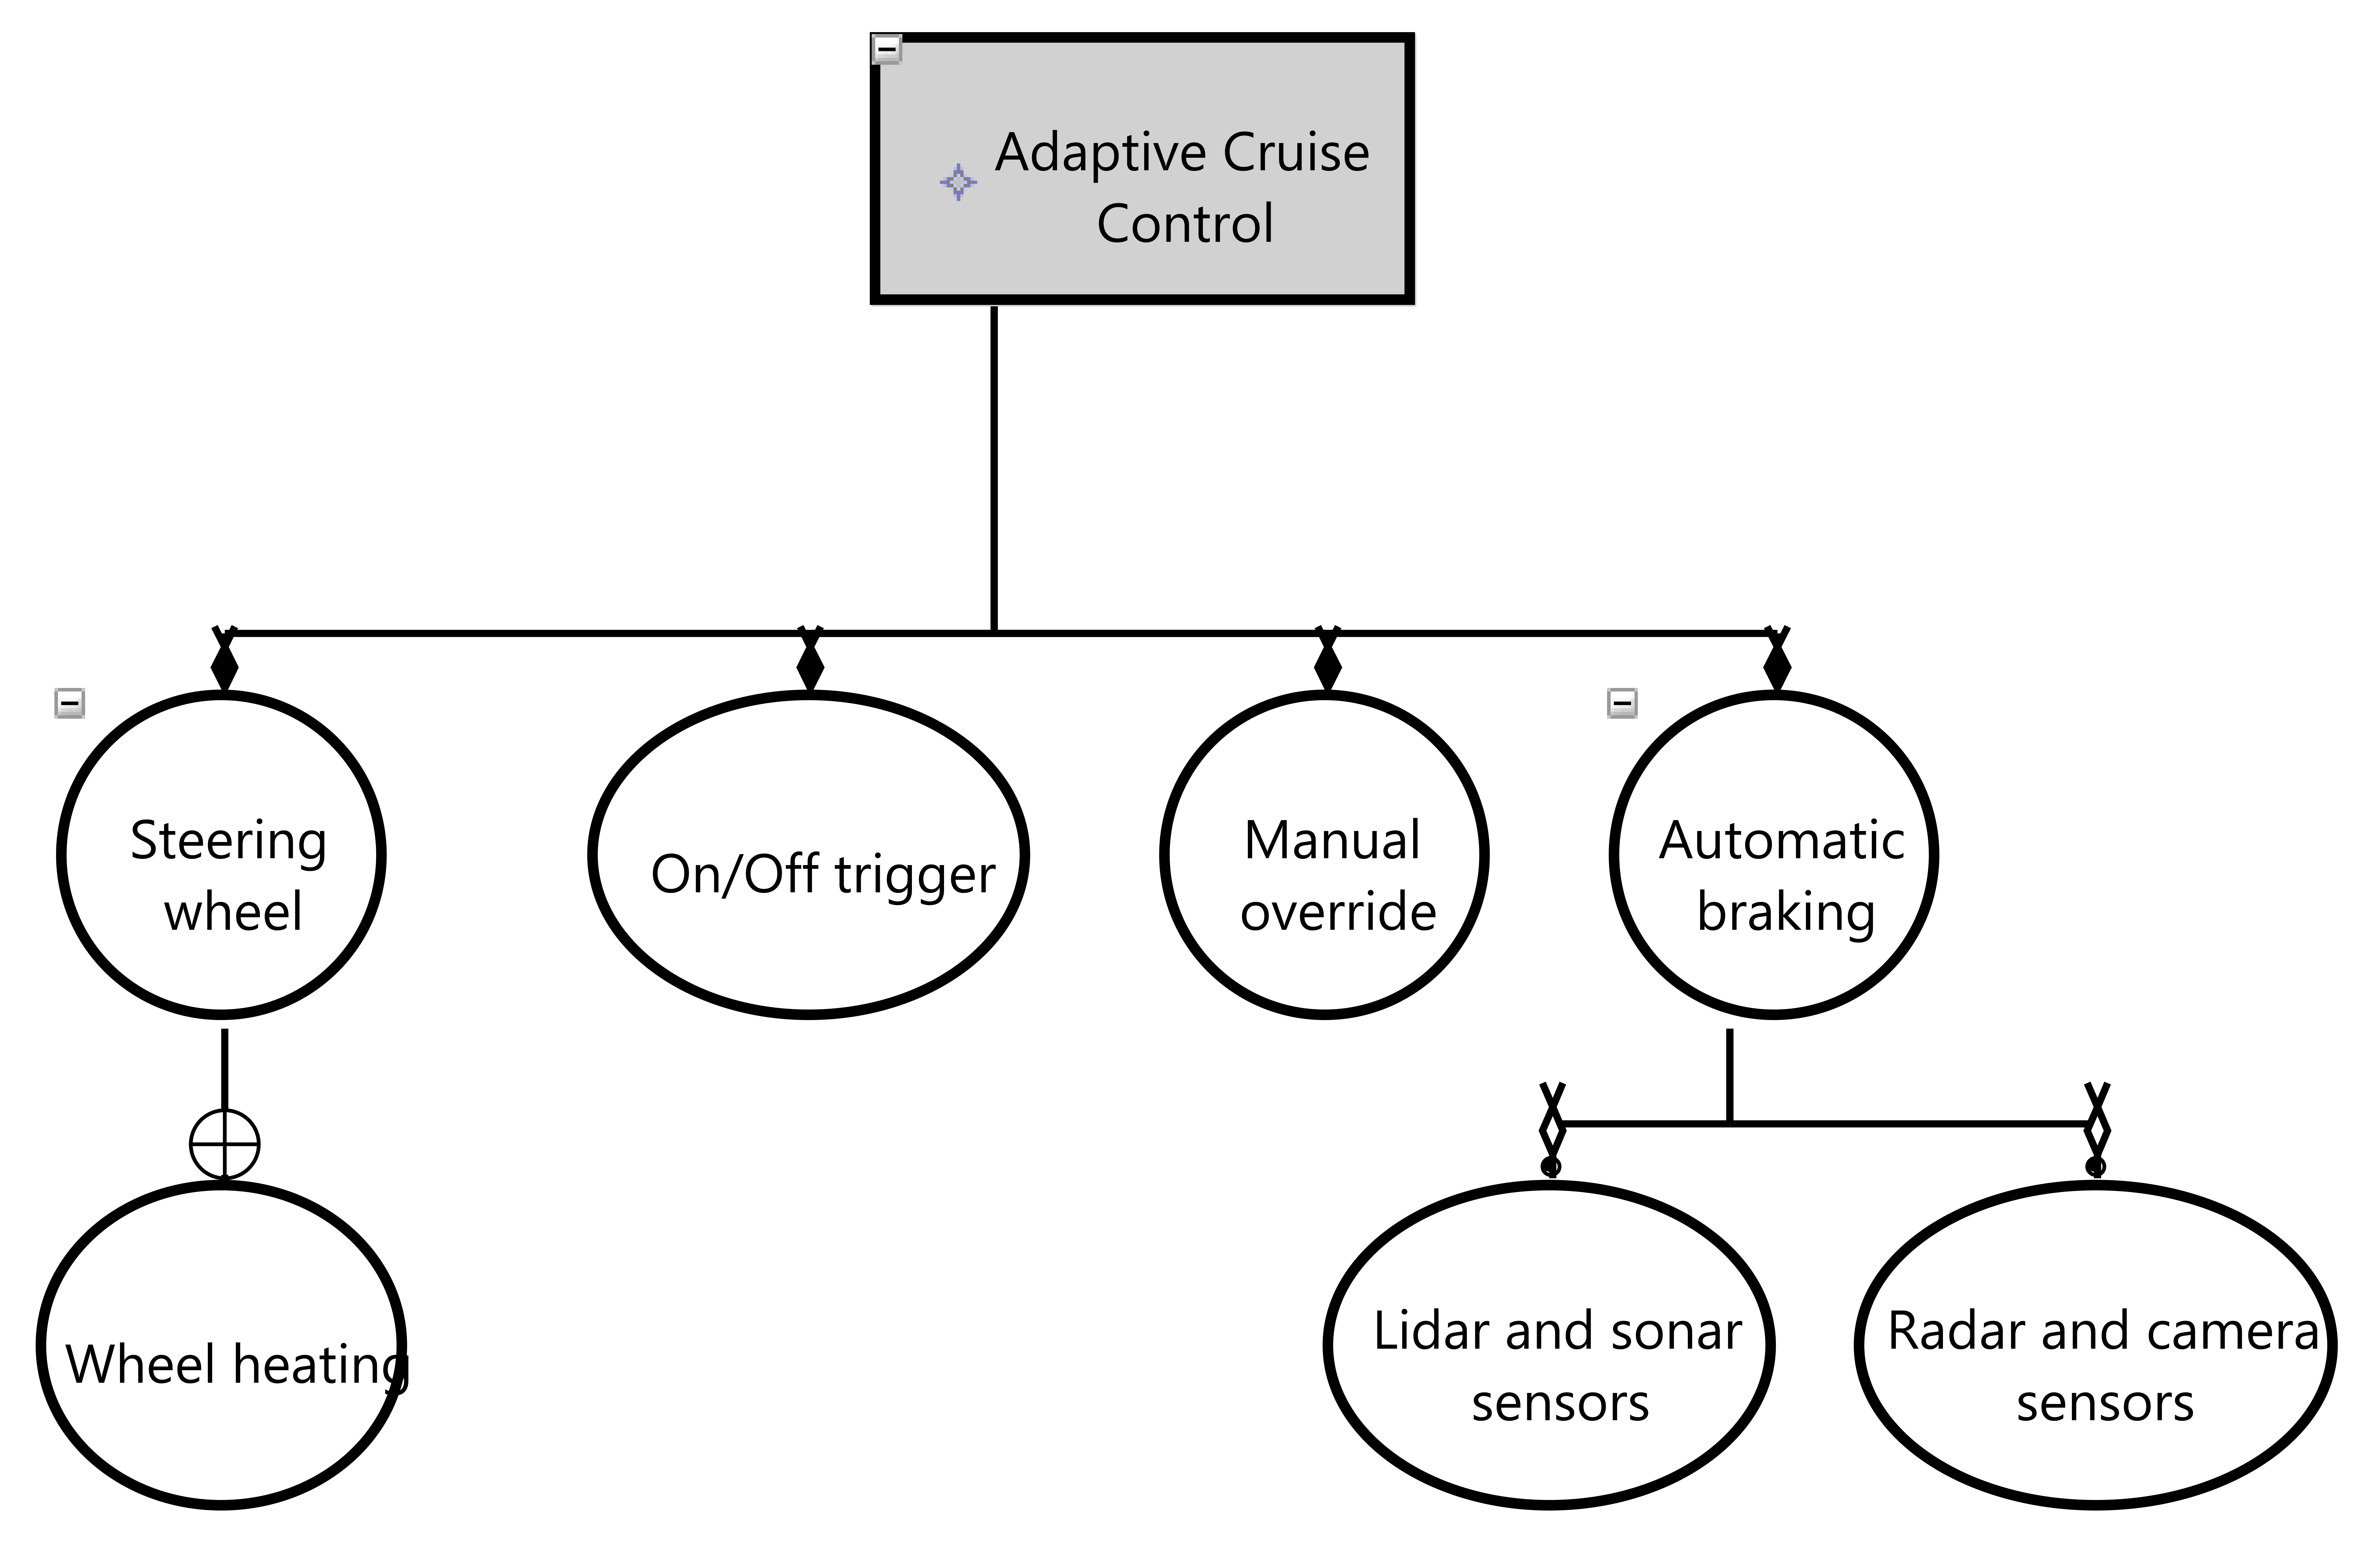
\includegraphics[width=\textwidth]{feature_model_acc.png}
	\caption{An example of the concrete syntax for the feature model using features for an adaptive cruise control system from the automotive domain.}
	\label{fig:concrete_syntax_feat_mod}
\end{figure}

Along with the graphical portion of \tool, we also implemented an Xtext-based~\cite{eysholdt2010xtext} specification language. The implemented specification language is based on the Gherkin specification language~\cite{nicieja2017writing, cucumberdocs}. We chose this as the specification language for our requirements for a few reasons. Gherkin uses a structured natural language for specifications, thus making it relatively approachable for users when defining their requirements. Further, despite using natural language, it uses keywords to provide a predicate logic structure to the specifications. The keyword `Given' is used for preconditions, `When' is used for events, and `Then' is used for postconditions. The combined approach of adding predicate structure to natural language makes it relatively easy to specify requirements and to implement the language within \tool. This helps to satisfy the ease of use and adoption requirement as it makes the tool more approachable to learn and implement in a development process. We found that Gherkin struck a nice balance between formal informal approaches to specification that aligns with the philosophy presented in Meyer's requirement style that inspired some of this methodology.

\begin{figure}
	\begin{lstlisting}
		Given{
			Precond FeatureExists: "Steering wheel has heating feature."
			Precond CarIsOn: "Vehicle is on."
		}
		When{
			Event UserTurnsOnHeating: "User interacts with heating interface to turn on/off wheel heating."
		}
		Then{
			Postcond StateChange: "Wheel heating boolean changes state to on or off depending on current state."
		}
	\end{lstlisting}
	\caption{Gherkin specification for Wheel Heating on/off functional requirement. The high-level requirement description is: User shall be able to turn wheel heating on/off.}
	\label{fig:specification}
\end{figure}

\section{Design Decisions}

A major design decision for \tool\ was using our own design for feature modelling. Other tools such as FeatureIDE already exist and are native to Eclipse. We decided to use our own implementation to remove possible constraints of having to work with an existing tool so that we can focus on the traceability aspects of the tool. Another reason was to allow us some flexibility in how to implement the new hierarchical relationship between features and requirements. Further, this gave us flexibility to explore how we might want to navigate the created models and traceability matrices. 

\subsection{Composition Implementations}

The relationship between features and requirements makes traditional composition techniques for \ac{PLE} a challenge. Given our convention that a variant requirement necessitates a new feature, the path to composing features and requirements to a product is relatively straightforward at this time. Currently, the approach focuses on the features themselves for the composition, with the assumption that each feature has unique requirements. If a requirement applies to multiple features then it is meant to be abstracted up a level in the tree to a higher feature. This currently reduces cross cutting concerns and dependencies between requirements. This allows users to define the necessary constraints and rules for how the features within a model are allowed to compose to a product (every car needs 4 wheels for example). As of the time of writing more complex analysis is planned for future work, however as a proof of concept, \tool\ has the facilities to support such development in the future. With the \texttt{Product\_Variant} class in the metamodel~\ref{fig:metamodel} we provide the facilities for a user to manually create instances of their product. Also due to the composition relationship that we use, all the product instances are owned by the feature model they are created in. The inheritance relationship also means that they don't need to be new semantic elements to represent the various features and requirements in the product variants. We can take advantage of model slicing to create those new variants and instances. Naturally, the inheritance also allows all the traceability mechanisms to apply to the product variants the same way they do to the parent feature model.

\section{Summary}
In summary, the tool for \tool\ has shown promise for enforcing the syntax and semantics we desire. We were able to implement the concrete syntax while maintaining a bijective relationship between the definitions in the metamodel and the concrete syntax in the tool. Our design decisions were justified and we were able to satisfy our tool objectives we outlined before beginning development of the tool. In the next chapter we will be exploring a preliminary analysis of the capabilities of the implementation. 